%%%%% Elektrisches Feld %%%%%
%% # Braunsche Röhre %%


%Some sample text to be displayed above the first subsection

%\subsection{Prinzip}

%Ein Zyklotron besteht aus Zwei hohlen, halbzylindrischen und Duanden an denen eine Spannung mit unterschiedlichem Vorzeichen anliegt, und darüber bzw. darunter liegende Magneten, die ein homogenes Magnetfeld erzeugen. Zudem gibt es einen Einlass und einen Auslass für Teilchen.

%\begin{wrapfigure}{r}{0.4\textwidth} \label{Zyklo}
%
%	\vspace{-10pt}
%	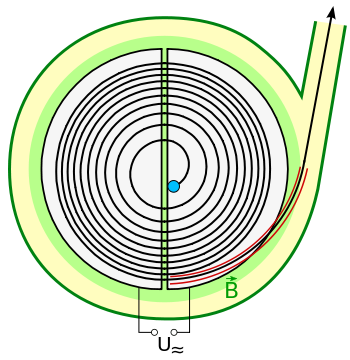
\includegraphics[width=0.35\textwidth]{Zyklotron_Prinzipskizze02.png}
%	\vspace{-13pt}
%	\caption{Prinzipskizze eines Zyklotrons}
%	\vspace{-5pt}	
%	
%\end{wrapfigure}

%\subsubsection{Anwendung}

% Some Formula:

%\begin{equation}
%	x= \frac{y \cdot 13 \pi z}
%			{\cos \alpha}
%\end{equation}

%%%%%%%%%%%%%%%%%%%%%%%
% Eigentlicher Beginn %
%%%%%%%%%%%%%%%%%%%%%%%

Eine Braun'sche Röhre wird z.B. Bildschirm eines Oszilloskopes verwendet. Ihre Aufgabe ist es, beschleunigte Elektronen seitlich so abzulenken, sodass diese auf einer bestimmten Stelle auf einem dahinter liegenden Schirm auftreffen und dort durch eine Leuchtschicht, die durch das Auftreffen von Elektronen zum Leuchten angeregt wird, sichtbar gemacht werden.

\subsection{Aufbau und Funktionsweise}

Zu Beginn müssen zunächst freie Elektronen erzeugt werden. Dies geschieht über einen Glühwendeln, ein gewickelter Draht durch den ein hoher Strom fließt. Dadurch glüht er und sondert gemäß dem glühelektrischen Effekt\footnote{Siehe auch: \url{https://de.wikipedia.org/wiki/Edison-Richardson-Effekt}} ab.

Diese Elektronen werden nun mit dem elektrischen Feld einer positiv geladenen Platte beschleunigt und durch eine Lochscheibe in einen oder zwei Kondensatoren geleitet.

In diesen Kondensatoren erfolgt die eigentliche Ablenkung, gemäß der Elektronenbewegung in elektrischen Feldern (siehe: \referenz{sec:BewegungsgesetzElektronen}). Um einen zwei-dimensionalen Schirm zu bestrahlen, müssen zwei Kondensatoren interagieren. Für jegliche Berechnung spart man sich dies allerdings und betrachtet nur die Ablenkung in einem Kondensator. Siehe dazu die Abbildung \ref{fig:BraunscheRoehre} \footnote{Abbildung von \url{http://www.abi-physik.de/buch/das-elektrische-feld/braunsche-roehre/}}.

\begin{figure}[h!] 
	\centering
	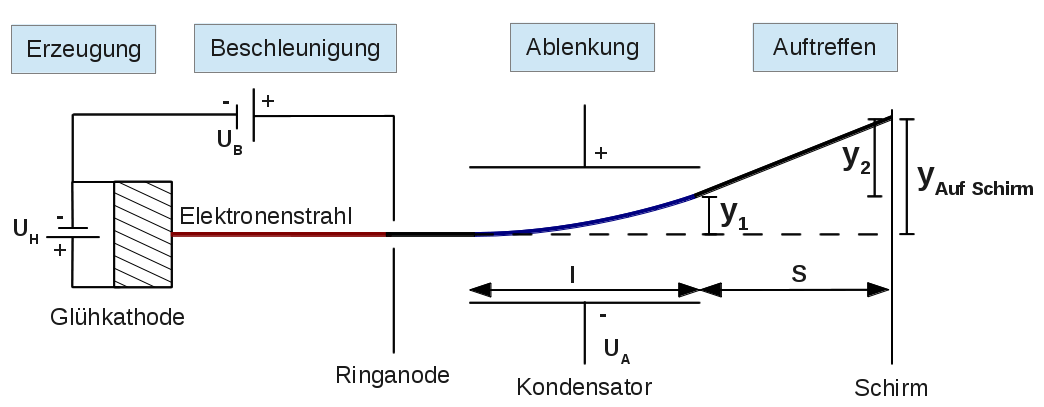
\includegraphics[width=0.9\textwidth]{Braun}
	\caption{Schema einer Braun'schen Röhre}
	\label{fig:BraunscheRoehre}
\end{figure}

\subsection{Mathematisierung}

\subsubsection{Beschleunigungsphase}

Um die auf die endgültige Geschwindigkeit der beschleunigten Elektronen zu schließen, lässt sich ein Energieansatz vollziehen. Die generelle kinetische Energie $E_{kin}=\frac{1}{2}m \cdot v^2$ (wichtige Formel, die allgemein bekannt sein sollte) lässt sich der Energie des elektrischen Feldes $E_{el}=q \cdot U_B$, welches von der Platte ausgeht gleichsetzten. Dabei ist zudem $q = e$ und $m = m_e$, da wir es mit Elektronen zu tun haben:

\begin{align} \label{eq:BeschleunigungNachV}
\begin{split}
	E_{kin} &= E_{el} \\
	\frac{1}{2}m_e \cdot v_{x}^2 &= e \cdot U_B \\
	v_x &= \sqrt{\frac{2e \cdot U_B}{m_e}}
\end{split}
\end{align}

\begin{leftbar}
Aufgabe: Oft ist die Endgeschwindigkeit gegeben sein und es ist nach der Spannung gefragt. Stelle die Gleichung nach U um! Solche Umformungen sind fast das Wichtigste in der Schulphysik.
\end{leftbar}

\subsubsection{Ablenkungsphase}

Die Bewegung in wieder aufgeteilt in eine gleichförmige Bewegung in x-Richtung und eine gleichmäßig beschleunigte Bewegung in y-Richtung. Da sich dies zudem in einem Kondensator abspielt können wir exakt die Gleichung \ref{eq:y(x)imKondensator} heranziehen. Allerdings muss zur Abgrenzung von der Beschleunigungsspannung der Ablenkspannung der Index $A$ zugefügt werden:

\begin{align} \label{eq:y_1(x)Braun}
\begin{split}
	y_1(x) &= \frac{e \cdot U_A}{2d \cdot m_e} \cdot \frac{x^2}{v_{x}^2}
\end{split}
\end{align}

Jetzt kann noch die Geschwindigkeit $v_{x}$ mit der Gleichung \ref{eq:BeschleunigungNachV} ersetzt werden:

\begin{align} \label{eq:y_1(x)BraunMitV}
\begin{split}
	y_1(x) &= \frac{e \cdot U_A}{2d \cdot m_e} \cdot \frac{x^2 \cdot m_e}{2e \cdot U_B} \\
	y_1(x) &= \frac{1}{4} \cdot \frac{U_A \cdot x^2}{d \cdot U_B}
\end{split}
\end{align}


\subsubsection{Exkurs: Nach Austritt aus Kondensator}

Die Bewegung nach dem homogenen elektrischen Feld bis zum Auftreffen auf dem Schirm ist die letzte Phase. Sie ist ebenfalls eine gleichförmige Bewegung, da die Elektronen in keiner Weise mehr beschleunigt werden. Allerdings besteht die Schwierigkeit hierbei, dass sie trotzdem in x und y-Richtung unterteilt werden muss (Das Elektron wurde in Phase 2 ja schon vertikal Abgelenkt). Daher muss neben der Geschwindigkeit in x-Richtung, welche über die gesamte Bahn des Elektrons konstant ist (Siehe: \gleichungsreferenz{eq:BeschleunigungNachV}), auch die Geschwindigkeit in y-Richtung, die am Ende der Ablenkphase erreicht wird, errechnet werden. 

Die Geschwindigkeit für gleichförmig beschleunigte Bewegungen allgemein (Bewegungsgesetze!) ist die Ableitung des Wegs:

\begin{align} \label{eq:v(t)Allgemein}
\begin{split}
	v_y(t) &= a \cdot t
\end{split}
\end{align}

\noindent Auf den Kontext angewendet gilt, mit $a = \frac{e \cdot U}{d \cdot m_e}$ (Vergleiche mit Gleichung \ref{eq:y_1(x)Braun}) und $t=\frac{x}{v_x}$:

\begin{align} \label{eq:v(x)Kontext}
\begin{split}
	v_y(x) &= \frac{e \cdot U_A}{d \cdot m_e} \cdot \frac{x}{v_x}
\end{split}
\end{align}

\noindent Um die Geschwindigkeit in y-Richtung im beim Austritt aus dem Kondensator zu berechnen, also bei dem Weg in x-Richtung, bei dem keine Beschleunigung mehr auf das Elektron wirkt, muss also die Länge des Kondensators gekannt werden und in die obige Gleichung eingesetzt werden. Sie wird hier mit $l$ abgekürzt:

\begin{align} \label{eq:v(t)Gesamt}
\begin{split}
	v_{y,Austritt} &= \frac{e \cdot U_A}{d \cdot m_e} \cdot \frac{l}{v_x}
\end{split}
\end{align}

\noindent Mit dieser Geschwindigkeit kann man das Bewegungsgesetz für das Elektron nach dem Austritt aus dem Kondensator aufstellen. Dafür kommt die gleichförmige Bewegung ($y(t) = v \cdot t$) zum Einsatz:

\begin{align} \label{eq:y(t)Gesamt}
\begin{split}
	y_2(t) &= v_{y,Austritt} \cdot t \\
	y_2(t) &= (\frac{e \cdot U_A}{d \cdot m_e} \cdot \frac{l}{v_x}) \cdot t \\
	y_2(x) &= (\frac{e \cdot U_A}{d \cdot m_e} \cdot \frac{l}{v_x}) \cdot \frac{x}{v_x} \\
	y_2(x) &= \frac{e \cdot U_A}{d \cdot m_e} \cdot \frac{l \cdot x}{v_{x}^2}
\end{split}
\end{align}

\subsubsection{Exkurs: Gesamtgleichung}

\noindent Mit dem Abstand des Schirmes von dem Ende des Kondensators ($s$) und der Beziehung für die Zeit $t=\frac{s}{v_x}$ vom Verlassen des Feldes bis zum Auftreffen auf den Schirm, kann eine Gesamtgleichung erstellt werden, die aus zwei Teilen besteht. Sie ist die Addition des Weges in y-Richtung zwischen dem Verlassen des Kondensators und dem Auftreffen auf den Schirm ($y_2(x=s)$, siehe Gleichung \ref{eq:y(t)Gesamt}) und des Weges in y-Richtung, der bereits beim Verlassen des Kondensators absolviert wurde ($y_1(x=l)$, siehe Gleichung \ref{eq:y_1(x)Braun}).

\begin{align} \label{eq:yGesamtAnsatz}
\begin{split}
	y_{Auf \ Schirm} &= y_1(x=l) + y_2(x=s) \\
	y_{Auf \ Schirm} &= \frac{e \cdot U_A}{2d \cdot m_e} \cdot \frac{l^2}{v_{x}^2}
				      + \frac{e \cdot U_A}{d \cdot m_e} \cdot \frac{l \cdot s}{v_{x}^2} \\
	y_{Auf \ Schirm} &= \frac{e \cdot U_A \cdot l}{d \cdot m_e \cdot v_{x}^2} \cdot (\frac{1}{2}l + s)
\end{split}
\end{align}

Als letzter Schritt wird noch $v_{x}$ durch $\sqrt{\frac{2e \cdot U_B}{m_e}}$ aus Gleichung \ref{eq:BeschleunigungNachV} ersetzt:

\begin{align} \label{eq:yGesamt}
\begin{split}
	y_{Auf \ Schirm} &= \frac{e \cdot U_A \cdot m_e}{d \cdot m_e \cdot 2e \cdot U_B} \cdot (\frac{1}{2}l + s) \\
	y_{Auf \ Schirm} &= \frac{1}{2} \cdot \frac{U_A \cdot l}{d \cdot U_B} \cdot (\frac{1}{2}l + s)
\end{split}
\end{align}

\begin{leftbar}
Anmerkung: Dieser Exkurs ist zwar interessant und das gekonnte Herleiten und Umstellen von Gleichungen ist in der Physik generell extrem wichtig, der Inhalt dieser Herleitung ist aber nicht klausurrelevant, dass heißt, es müssen keine Formel gelernt werden oder ähnliches. Trotzdem ist es eine anspruchsvolle und lehrreiche Aufgabe, diese Herleitung nachzuvollziehen und gegebenenfalls selbst zu vollführen.
\end{leftbar}




